% This is a LaTeX template for poster using University of Helsinki style
% This version uses pdflatex; if you have XeTeX available, consider using poster_xetex.tex for fancy font settings
%
% The official Graphical Instructions available from hy.logodomain.com (from university network only) defines colours, fonts etc. This Template does not perfectly match the official poster template of the university
%
% Jukka Suomela's collection of LaTeX tricks has been invaluable in building this template: http://cs.helsinki.fi/u/josuomel/latex/ 
%
% Template by Janne Korhonen
% Encoding of this file is iso-8859-1 latin 1

\documentclass[a4paper]{article} % This actually makes poster of size A4, scale up when printing. Used text font size is a bit small for A1 poster, preferably use \small in that case 

% Misc. packages
\usepackage[T1]{fontenc}
\usepackage{url}
\usepackage{amsfonts}
\usepackage[absolute]{textpos}
\usepackage{amssymb}
\usepackage{amsmath} 
\usepackage{amsthm}
\usepackage{listings}

% Graphics stuff
\usepackage[usenames,dvipsnames]{color}
\usepackage{graphicx}

% My favourite macros
\newcommand{\N}{\mathbb{N}} %natural numbers
\newcommand{\Z}{\mathbb{Z}} %integers
\newcommand{\Q}{\mathbb{Q}} %rationals
\newcommand{\R}{\mathbb{R}} %reals
\newcommand{\G}{\mathcal{G}} % fancy G
\newcommand{\A}{\mathcal{A}} % fancy A
\newcommand{\bO}{\mathcal{O}} % fancy O

% enumitem for controlling enumerate and itemize environments; usefull for saving space
\usepackage{enumitem}

% Fonts
%
% Palantino - Helvetica - Courier.
% I haven't really spent time to figure out how to best match the official university style with latex font packages, as I use XeTex myself...
\usepackage{mathpazo}
\linespread{1.10}
\usepackage[scaled]{helvet}
\usepackage{courier}

% Colours
\definecolor{sciorange}{RGB}{252,163,17}
\definecolor{unigray}{RGB}{140,140,140}

% Textpos to manually position blocks of text on the page
\usepackage[absolute]{textpos}

% We define 1 mm grid for positioning the text blocks on the page
% The idea is to leave 10 mm marginals to all sides; the three text columns are 60 mm wide with 5 mm space between columns.
\setlength{\TPHorizModule}{1mm}
\setlength{\TPVertModule}{1mm}

% The origin is set to right below the main title; this means that main title blocks have negative y-coordinate. There is actually no good reason for this, I just happened to do this that way.
\textblockorigin{10mm}{45mm}

% parindent is set to zero, because it looks better in posters
% you could also add some space between paragraphs here, but I use manual vertical spaces in this sample
\setlength{\parindent}{0pt}


\newcommand{\abs}[1]{\lvert#1\rvert}
\newcommand{\norm}[1]{\lVert#1\rVert}
\newcommand{\biglr}[1]{\bigl(#1\bigr)}
\newcommand{\Biglr}[1]{\Bigl(#1\Bigr)}
\newcommand{\ceil}[1]{\lceil #1 \rceil}
\DeclareMathOperator*{\argmin}{arg\,min}
\DeclareMathOperator*{\argmax}{arg\,max}

\definecolor{dkgreen}{rgb}{0,0.6,0}
\definecolor{gray}{rgb}{0.5,0.5,0.5}
\definecolor{mauve}{rgb}{0.58,0,0.82}

\lstset{frame=tb,
  language=Python,
  aboveskip=1mm,
  belowskip=1mm,
  showstringspaces=false,
  columns=flexible,
  basicstyle={\fontsize{8}{8}\ttfamily},
  numbers=none,
  numberstyle=\tiny\color{gray},
  keywordstyle=\color{blue},
  commentstyle=\color{dkgreen},
  stringstyle=\color{mauve},
  breaklines=true,
  breakatwhitespace=true,
  tabsize=2,
  morekeywords={yield},
  literate={0}{\textcolor{sciorange}{0}}{1}%
             {1}{\textcolor{sciorange}{1}}{1}%
             {2}{\textcolor{sciorange}{2}}{1}%
}

% Finally, the content
\begin{document}
  \pagestyle{empty} % To get rid of page numbers and so
  % ------------------------------------------------------------------------
  % Main title, University logo etc.

  % If you need more space for the title or want the logo to be bigger, you need to adjust various parameters, as I did not bother to automate this yet
  % Mainly, move the textblockorigin above down and adjust all the boxes here to be higher up.

  % First, the University logo. The included flame.pdf is a copy of the official logo in vector format, so it is good for all sizes.
  % Box starts 10 mm from the top
  \begin{textblock}{95}(0,-35)
    
\includegraphics[width=22mm]{flame.pdf}
  \end{textblock}	

  % University - Faculty - Department
  % Box starts 10 mm from the top
  \begin{textblock}{95}(95,-35)
    {\fontsize{8}{7}\selectfont\sffamily\color{unigray}
    \hfill HELSINGIN YLIOPISTO

    \hfill HELSINGFORS UNIVERSITET

    \hfill UNIVERSITY OF HELSINKI

    \color{sciorange}\hfill MATEMAATTIS-LUONNONTIETEELLINEN TIEDEKUNTA

    \hfill MATEMATISK-NATURVETENSKAPLIGA FAKULTETEN

    \hfill FACULTY OF SCIENCE % For some reason, the last line here gets messed up without extra spaces...

    }
  \end{textblock}


  % Main title
  % If you need two lines for the title, you need to adjust the position of this block and textblockorigin
  % Remember, two first words use faculty colour. If your title is long, you can use small letters.
  \begin{textblock}{190}(0,-10)
    {\sffamily\huge{\color{sciorange}EXPERIMENTAL COMPARISON }{\color{unigray} OF MULTIPLE EXACT\vspace{1mm}\\STRING MATCHING ALGORITHMS}}
    \small\hfill Paul Saikko\\ % If you have multiple authors, their names can be on the same line. Adjust font size as necessary
    \rule[2mm]{190mm}{0.3pt} % This is the line under the title, adjust the last parameter if it seems to be in the wrong place
  \end{textblock}

  % ------------------------------------------------------------------------
  % The "abstract" block. Does not actually exist in the university poster template, so you may consider not using this
  \begin{textblock}{190}(0,6)
    \sffamily
    \small The \emph{multiple exact string matching} problem asks us to search a text $T$ of length $n$ for a set of patterns $\mathcal{P}$ with total length $\norm{\mathcal{P}}=m$. Obviously we could search the text for each pattern in $P$ using some exact string matching algorithm, but much better algorithms for this task exist. Here we give an overview of three such algorithms: Aho-Corasick, Shift-And, and Karp-Rabin. Each provides a different approach to solving the problem. We compare the theoretical performance of these algorithms to experimental results and attempt to identify the strenghts and weaknesses of each approach, assuming a constant alphabet size of $\sigma$ and equal-length patterns, $\abs {P_j}  = l$ for every $P_j \in \mathcal P$.
    
  \end{textblock}

  % Large subtitle with line. Again, not from the university template.
  \begin{textblock}{190}(0,28)
    \sffamily
    \Large{\color{sciorange}THE ALGORITHMS}\small\\
    \rule[3mm]{190mm}{0.1pt}
  \end{textblock} 

  % ------------------------------------------------------------------------
  % Three-column stuff
  %
  % The vertical size of the columns depends on the content, so unfortunately you have to manually move contents around

  % First column
  \begin{textblock}{60}(0,35)
    {\sffamily\normalsize{\color{sciorange}AHO-CORASICK}}\vspace{1mm}\\ % Titles among the main text are made like this, not by using \section
    \footnotesize
      \textbf{The algorithm.} We can construct a trie from the patterns $\mathcal P$, then for each node, add a link to the node that represents the longest proper suffix of the node and make note of pattern occurrences. The automaton can be then simulated with the text $T$ as input to find occurrences.\vspace{1mm}\\
      \textbf{Aho-Corasick automaton.} For the patterns \\
      $\mathcal P = \{\text{he},\text{she},\text{his},\text{hers}\}$
      we can produce the following automaton:\\
      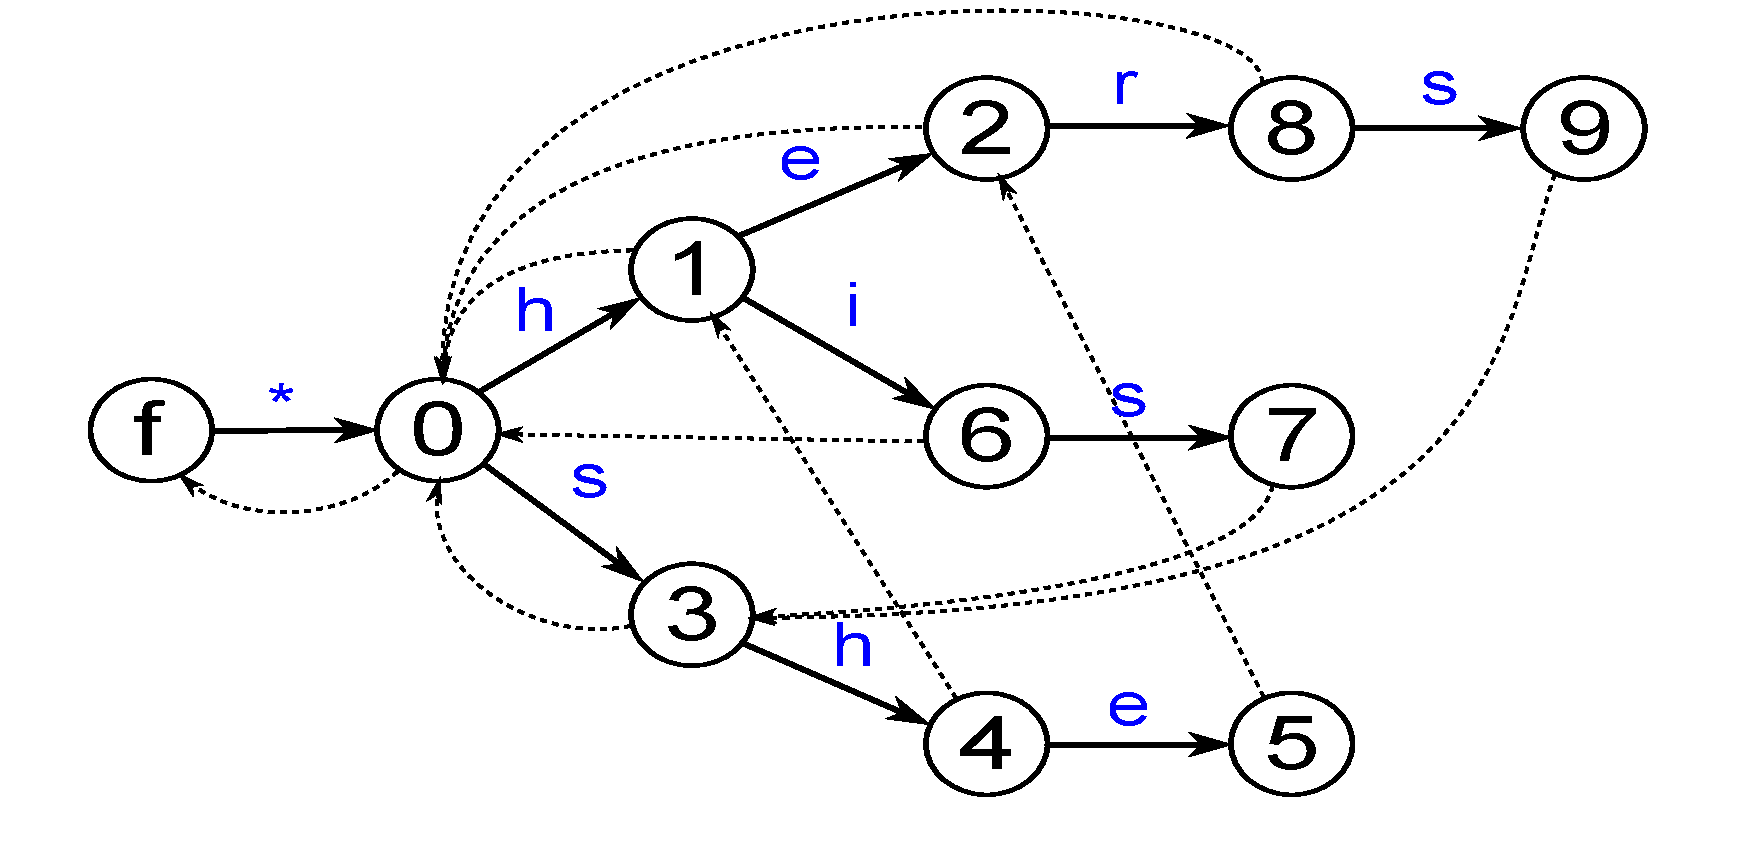
\includegraphics[width=60mm]{AC-automaton.pdf}
      \textbf{Time complexity.}
      \begin{itemize}[labelindent=2mm,leftmargin=*,itemsep=1mm, topsep=1mm]
        \item Preprocessing: $O(m)$
        \item Search: $O(n)$
      \end{itemize}
  \end{textblock} 
  
  % Second column
  \begin{textblock}{60}(65,35)
    {\sffamily\normalsize{\color{sciorange}SHIFT-AND}}\vspace{1mm}\\
    \footnotesize 
      \textbf{The algorithm.} Shift-And scans the text, it maintaining a bitvector D which keeps track of the longest prefixes of patterns it has encountered. 
\begin{lstlisting}[mathescape]
# preprocessing      
for (i = 0; i < m; i++):
  B[P[i/l][i%l]] += 2${}^i$
for (i = 0; i < m; i += l): 
  pBegin += 2${}^i$
for (i = l - 1; i < m; i += l): 
  pEnd += 2${}^i$
# search      
for (i = 0; i < n; i++):
  D = ((D << 1) | pBegin) & B[T[i]]
  if D & pEnd $\neq$ 0: yield i
\end{lstlisting}
      \textbf{Bitparallelism.} The bitvectors D, pBegin, and pEnd can be represented in $\ceil {m/w}$ machine words. B can be stored in $\sigma\ceil {m/w}$ and D can be updated in $O(\ceil {m/w})$ bitwise operations at each step. \vspace{1mm}\\
      \textbf{Time complexity.}
      \begin{itemize}[labelindent=2mm,leftmargin=*,itemsep=1mm, topsep=1mm]
        \item Preprocessing: $O(m)$
        \item Search: $O(n \lceil m / w \rceil)$
      \end{itemize}
  \end{textblock}

  % Third column
  \begin{textblock}{60}(130,35)
    {\sffamily\normalsize{\color{sciorange}KARP-RABIN}}\vspace{1mm}\\
    \footnotesize 
      \textbf{Karp-Rabin hash function.} For some fixed positive integers $r$ and $q$, the karp-rabin hash of a string 
      $S = s_0 s_1 \dotsc s_{m-1}$ is 
      $$ H(S) = \sum_{i=0}^{m-1} (s_i r^{m-1-i})\mod q. $$
      This is an example of a rolling hash function -- if we know the hash $H(T_{[i\dotsc i+m]})$, 
      we can compute $H(T_{[i+1\dotsc i+1+m]})$ in constant time.\vspace{1mm}
      
      \textbf{Multiple string matching.} We can precompute the hash value for every pattern and store them in a data structure that supports constant-time lookups. Potential occurrences in the text can be found by computing $H(T_{[i\dotsc i+l]})$ for each $i \in [0\dotsc n-l)$, and comparing them to the precomputed pattern hashes. Every potential occurrence must be checked, which leads to poor worst-case behavior.
      \vspace{1mm}
      
      \textbf{Average time complexity.}
      \begin{itemize}[labelindent=2mm,leftmargin=*,itemsep=1mm, topsep=1mm]
        \item Preprocessing: $O(m)$
        \item Search: $O(n+m)$
      \end{itemize}
  \end{textblock}

  % ----------------------- LOWER PART ----------------------------
  
  \begin{textblock}{190}(0,120)
    \sffamily
    \Large{\color{sciorange}EXPERIMENTAL RESULTS}\small\\
    \rule[3mm]{190mm}{0.1pt}
  \end{textblock} 

  \begin{textblock}{60}(0,127)
    {\sffamily\normalsize{\color{sciorange}METHODOLOGY}}\vspace{1mm}\\
    \footnotesize
      \textbf{Implementations.} The algorithms introduced above were implemented with java version 1.7. The source code for the implementations can be viewed on github at \url{https://github.com/psaikko/string-algorithms-project}.
      \vspace{1mm}\\
      \textbf{Experiments.} The experiment data was gathered using python scripts to automate running the algorithms. Every plotted data point is an average of 10 runs of the algorithm.
      \vspace{2mm}\\
    {\sffamily\normalsize{\color{sciorange}COMPARISON WITH THEORETICAL\\PERFORMANCE}}\vspace{1mm}\\
    \footnotesize 
      \textbf{With constant text length.} We plot the preprocessing and search times for each algorithm as the number of patterns to search for is increased.\\
      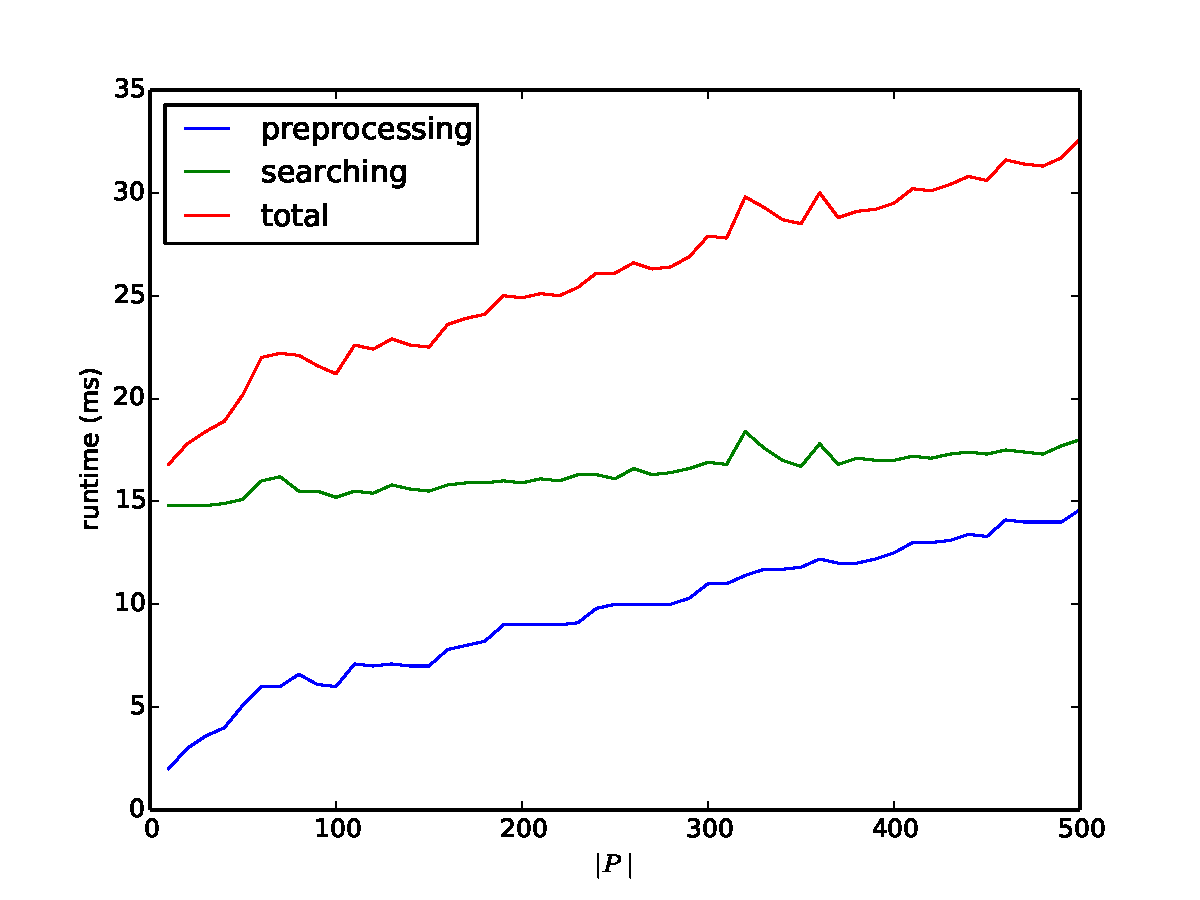
\includegraphics[width=60mm]{patterncount_Aho-Corasick.pdf}
      \textbf{Aho-Corasick.} We see search time staying roughly constant as expected, while preprocessing time increases linearly as we add more patterns.
  \end{textblock} 

  \begin{textblock}{60}(65,130)
    \footnotesize      
      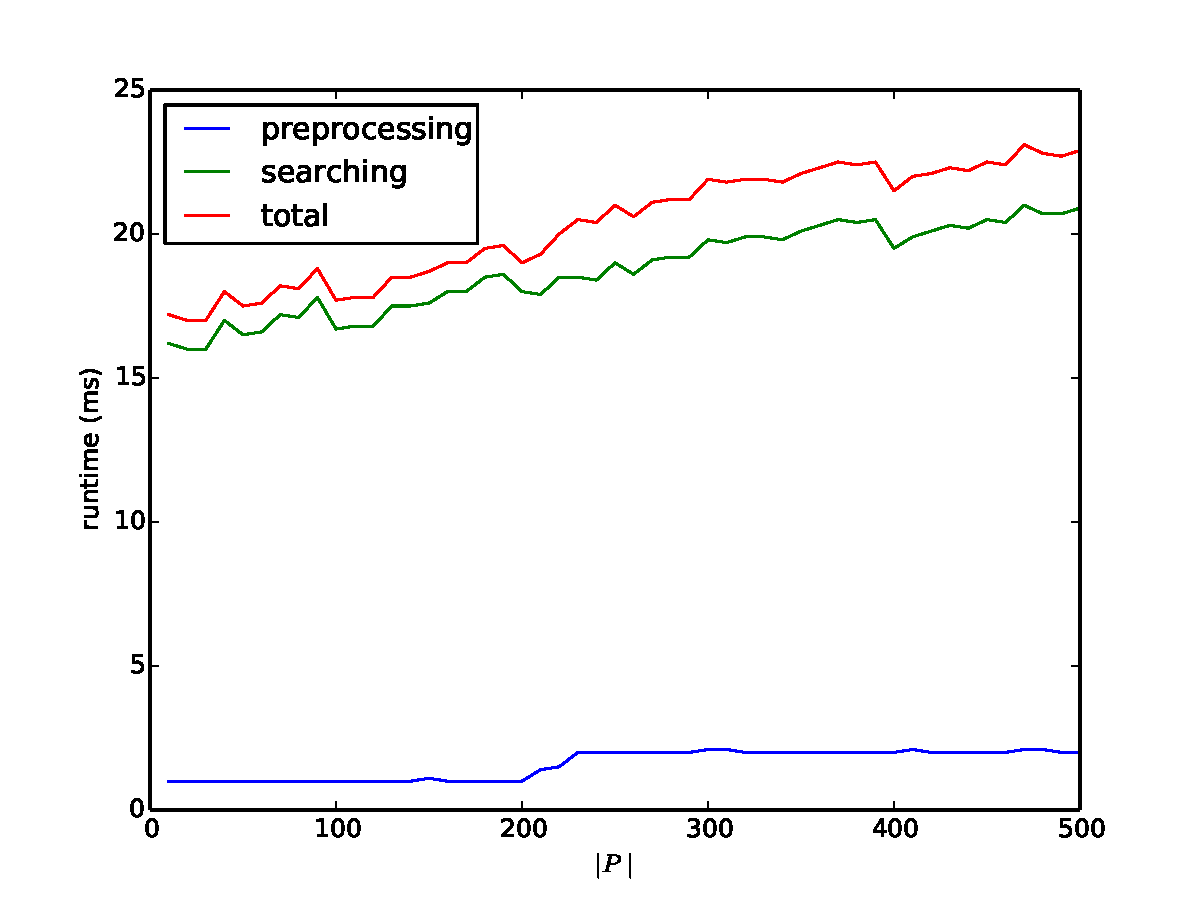
\includegraphics[width=60mm]{patterncount_Karp-Rabin.pdf}
      \textbf{Karp-Rabin.} The algorithm generally performs well despite poor worst-case behavior for search, preprocessing is quite fast.\\
      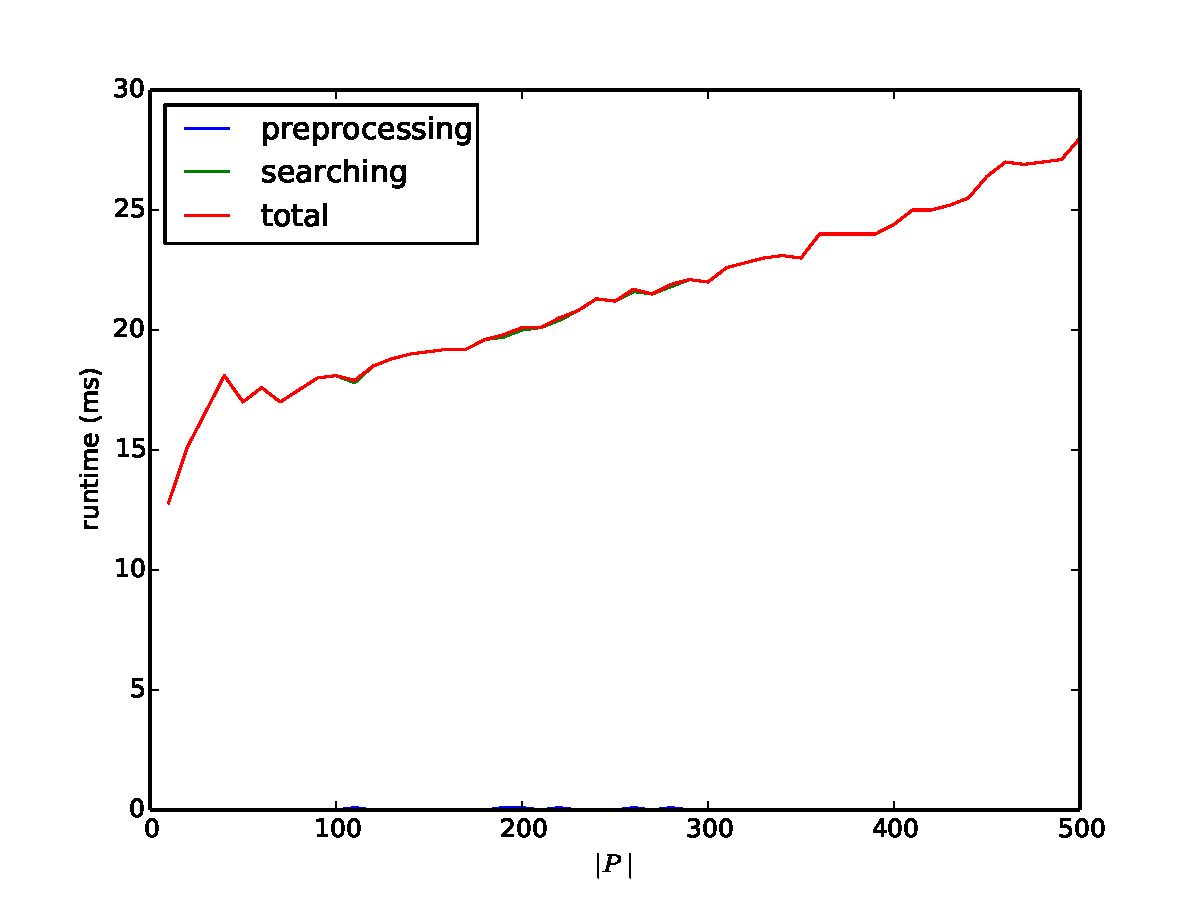
\includegraphics[width=60mm]{patterncount_Shift-And.pdf}
      \textbf{Shift-And.} The preprocessing time for Shift-And is much shorter than the other algorithms, despite the same asymptotic time complexity.\\
  \end{textblock}

  \begin{textblock}{60}(130,127)
    {\sffamily\normalsize{\color{sciorange}EDGE CASES}}\vspace{0.2mm}\\
    \footnotesize 
      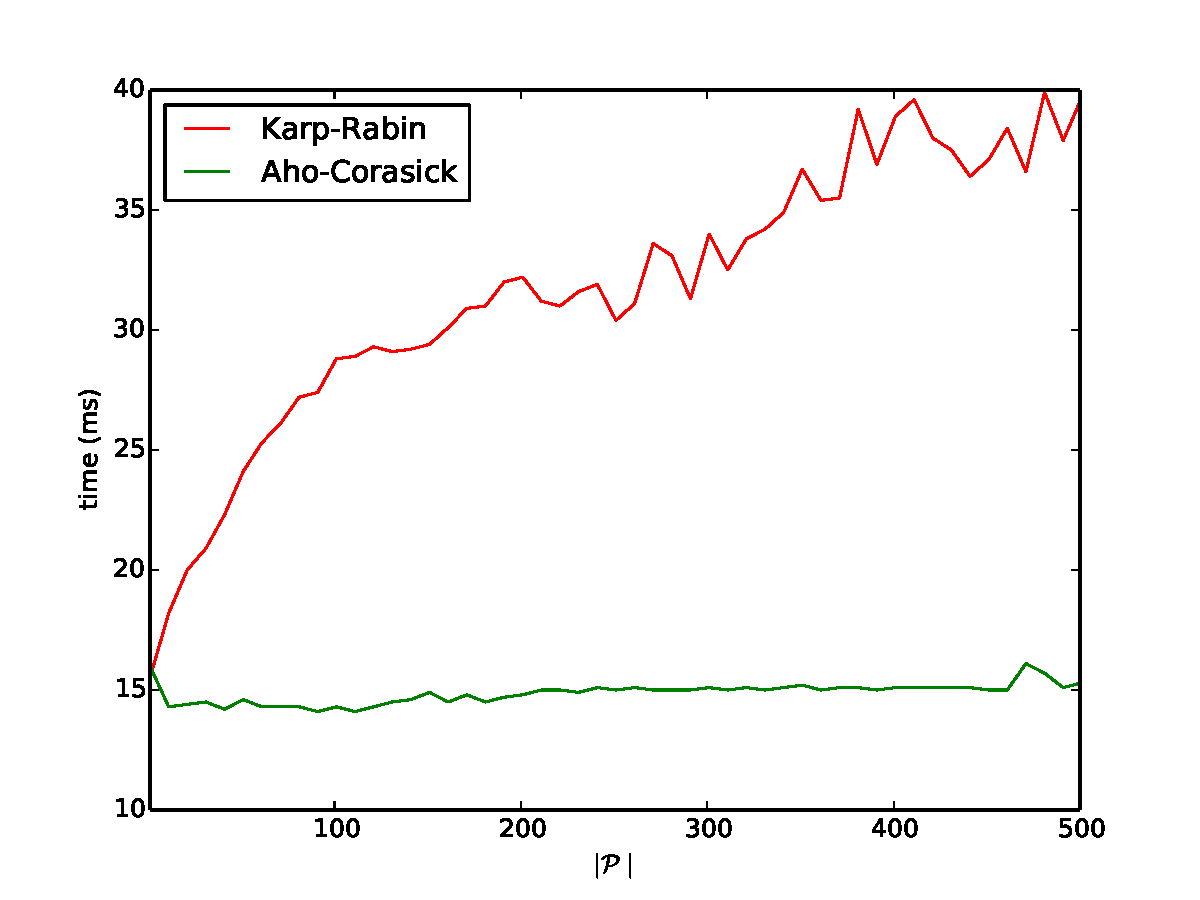
\includegraphics[width=60mm]{KRvAC.pdf}\\
      \textbf{Many short patterns.} A combination of the Karp-Rabin algorithm's $O(n+m)$ time complexity and hash collisions leads it to perform poorly.\\
      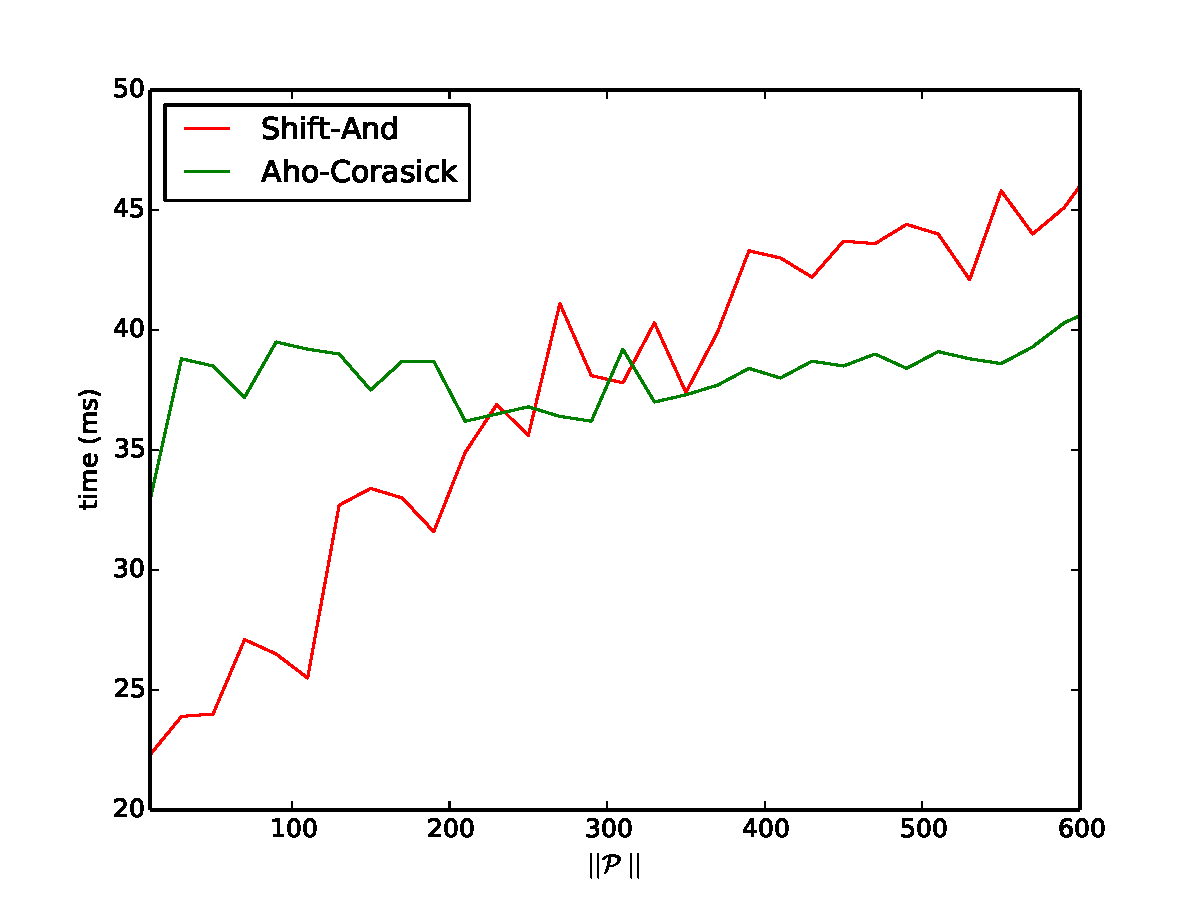
\includegraphics[width=60mm]{SAvAC.pdf}\\
      \textbf{Small total pattern length.} Although Shift-And scales poorly with total pattern length, the bitparallel algorithm is fast when $\norm{\mathcal P}$ is not large.
  \end{textblock}
% Unfortunately, this template has no references. The official instructions seem to indicate that sans-serif font is used for the reference list.
\end{document}
